\documentclass{beamer}

\usepackage{beamerthemesplit}
\usepackage{verbatim}
\usepackage[normalem]{ulem}

\usepackage{xcolor}

\usepackage{hyperref}

\definecolor{gold}{rgb}{1.,0.84,0.}
\definecolor{brightred}{rgb}{1.,0.4,0.4}
\definecolor{mygray}{RGB}{200,200,200}
\definecolor{lightsteelblue}{RGB}{176,196,222}
\definecolor{lightskyblue}{RGB}{135,206,250}
\definecolor{cadetblue}{RGB}{95,158,160}

\usetheme{default}
\usecolortheme{mule}

\usefonttheme{serif}

%\DeclareGraphicsExtensions{.pdf,.png,.jpg}

\newcommand{\mcal}{\textsc{metacalibration}}
\newcommand{\Mcal}{\textsc{Metacalibration}}

\newcommand{\mcalR}{\mbox{\boldmath $R$}}
\newcommand{\mcalRscalar}{\mbox{$R$}}

\newcommand{\mcalRmean}{\mbox{\boldmath $\langle R \rangle$}}
\newcommand{\mcalRscalarmean}{\mbox{$\langle R \rangle$}}

\newcommand{\mcalRpsf}{$R^{p}$}
\newcommand{\mcalRpsfnoise}{$R^{p}_\eta$}
\newcommand{\mcalRo}{\mbox{\boldmath $R_o$}}
\newcommand{\mcalRnoise}{\mbox{\boldmath $R_\eta$}}

\newcommand{\mcalRmeanalpha}{\mbox{\boldmath $\langle R_\alpha \rangle$}}
\newcommand{\mcalRmeanbeta}{\mbox{\boldmath $\langle R_\beta \rangle$}}

\newcommand{\mcalRg}{\mbox{\boldmath $R_\gamma$}}
\newcommand{\mcalRS}{\mbox{\boldmath $R_S$}}
\newcommand{\mcalRgmean}{\mbox{\boldmath $\langle R_\gamma \rangle$}}
\newcommand{\mcalRSmean}{\mbox{\boldmath $\langle R_S \rangle$}}

\newcommand{\mcalRtwopt}{\mbox{\boldmath $R^{2pt}$}}
\newcommand{\mcalRtwoptmean}{\mbox{\boldmath $\langle R^{2pt} \rangle$}}


\newcommand{\mcalRmodel}{\mbox{\boldmath $R^{model}$}}
\newcommand{\mcalRnoisemodel}{\mbox{\boldmath $R^{model}_\eta$}}


\newcommand{\vecg}{\mbox{\boldmath $\gamma$}}
\newcommand{\vest}{\mbox{\boldmath $e$}}

\newcommand{\snr}{$S/N$}
\newcommand{\snT}{$(S/N)_{\textrm{size}}$}
%\newcommand{\snT}{$\left( \frac{S}{N}\right)_{\textrm{size}}$}
\newcommand{\snflux}{$(S/N)_{\textrm{flux}}$}
%\newcommand{\snflux}{$\left( \frac{S}{N}\right)_{\textrm{flux}}$}

\newcommand{\lensfit}{\texttt{LENSFIT}}
\newcommand{\numba}{\texttt{Numba}}
\newcommand{\python}{\texttt{Python}}
\newcommand{\ngmix}{\texttt{ngmix}}
\newcommand{\shear}{{\bf g}}
\newcommand{\redmapper}{redMaPPer}
\newcommand{\est}{$e$}


\newcommand{\prelim}{{\bf{\it Preliminary}}}

\newcommand{\panda}{PanDA}
\newcommand{\bigpanda}{BigPanDA}



\title{LSST and \bigpanda}
\author{Erin Sheldon}
\institute{Brookhaven National Laboratory}

% http://texblog.net/latex-archive/plaintex/beamer-footline-frame-number/
% to add the page (frame ) number and not screw up the bottom line
% works for split themes?
\expandafter\def\expandafter\insertshorttitle\expandafter{%
      \insertshorttitle\hfill%
        \insertframenumber\,/\,\inserttotalframenumber}

% suppress navigation bar
\beamertemplatenavigationsymbolsempty
\setbeamertemplate{footline}{}

\begin{document}

\frame{\titlepage}


\setbeamertemplate{background canvas}[vertical shading][bottom=mgray,top=mblack]

\frame
{
    \frametitle{Large Synoptic Survey Telescope (LSST)}

    \setbeamerfont*{itemize/enumerate body}{size=\Large}
    \setbeamerfont*{itemize/enumerate subbody}{parent=itemize/enumerate body}
    \setbeamerfont*{itemize/enumerate subsubbody}{parent=itemize/enumerate body}
 
    \begin{itemize}

        \item LSST Intro
        \item Dark Energy Science Collaboration
        \item Some computing we would like to do with 

    \end{itemize}

}


{

    \frame
    {
        \frametitle{Example Image to LSST Depths (from HSC)}
        \begin{center}
            \includegraphics[width=1.0\textwidth]{fig1e.jpg}
            \newline
        \end{center}

    }

}



\frame
{
    \frametitle{LSST}

    \setbeamerfont*{itemize/enumerate body}{size=\Large}
    \setbeamerfont*{itemize/enumerate subbody}{parent=itemize/enumerate body}
    \setbeamerfont*{itemize/enumerate subsubbody}{parent=itemize/enumerate body}
 
    \begin{itemize}

        \item Huge astronomical survey covering half the sky

        \item Diverse range of science: from cosmology,  supernovae, milky
            way science, solar system science

        \item Time domain component: revisit each part of the sky of order
            1000 times.

        \item Biggest camera ever made: 3.2 gigapixels.  BNL leads the
            development of the CCD sensors.

        \item Will generate 60 PB of imaging data.

    \end{itemize}

}

{

    \frame
    {
        \frametitle{LSST Camera}
     
        \begin{center}
            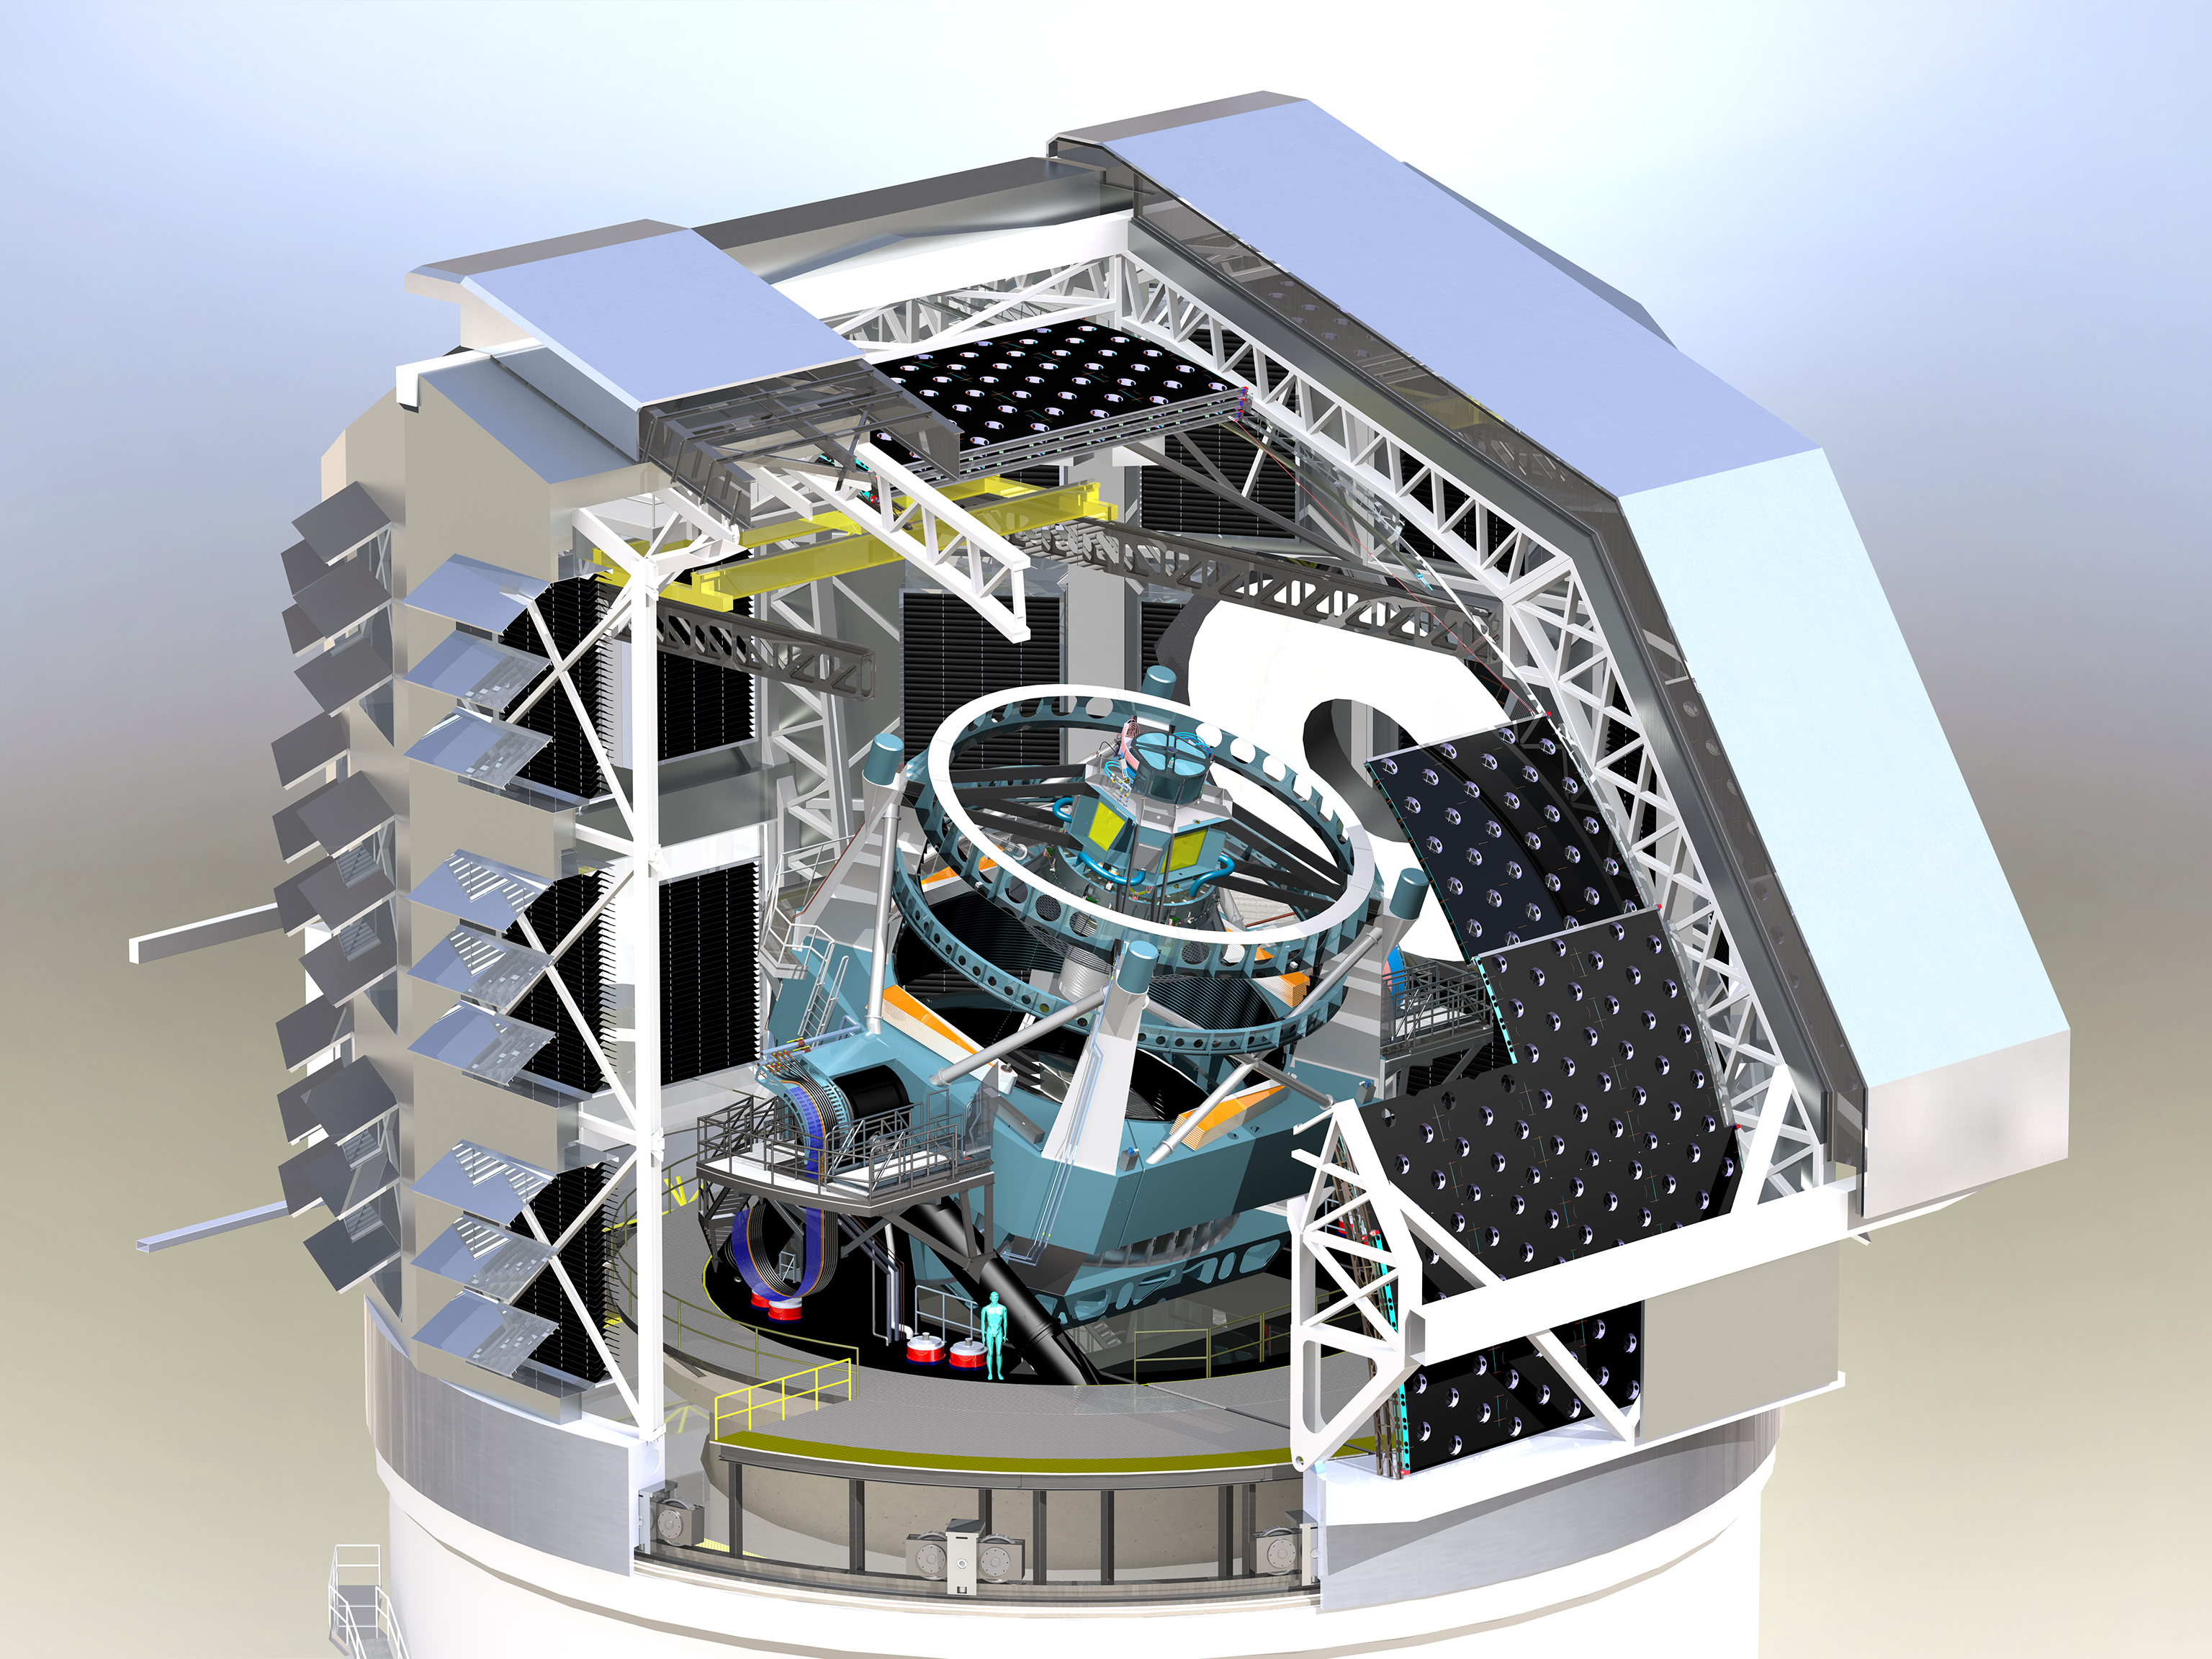
\includegraphics[width=0.9\textwidth]{Dome_and_Telescope_sm.jpg}
            \newline
        \end{center}

    }

}

{

    \frame
    {
        \frametitle{LSST Camera}
     
        \begin{center}
            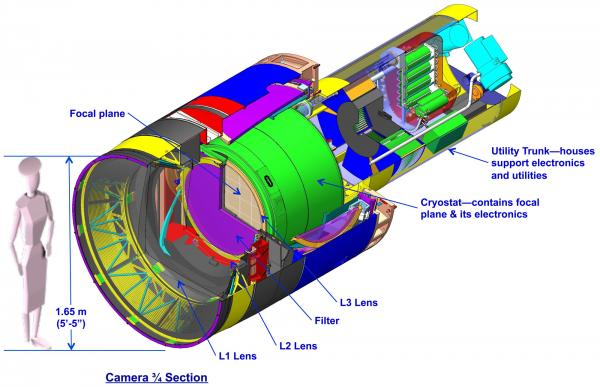
\includegraphics[width=0.9\textwidth]{Camera_Layout-full.jpg}
            \newline
        \end{center}

    }

}

{

    \frame
    {
        \frametitle{LSST Camera}
     
        \begin{center}
            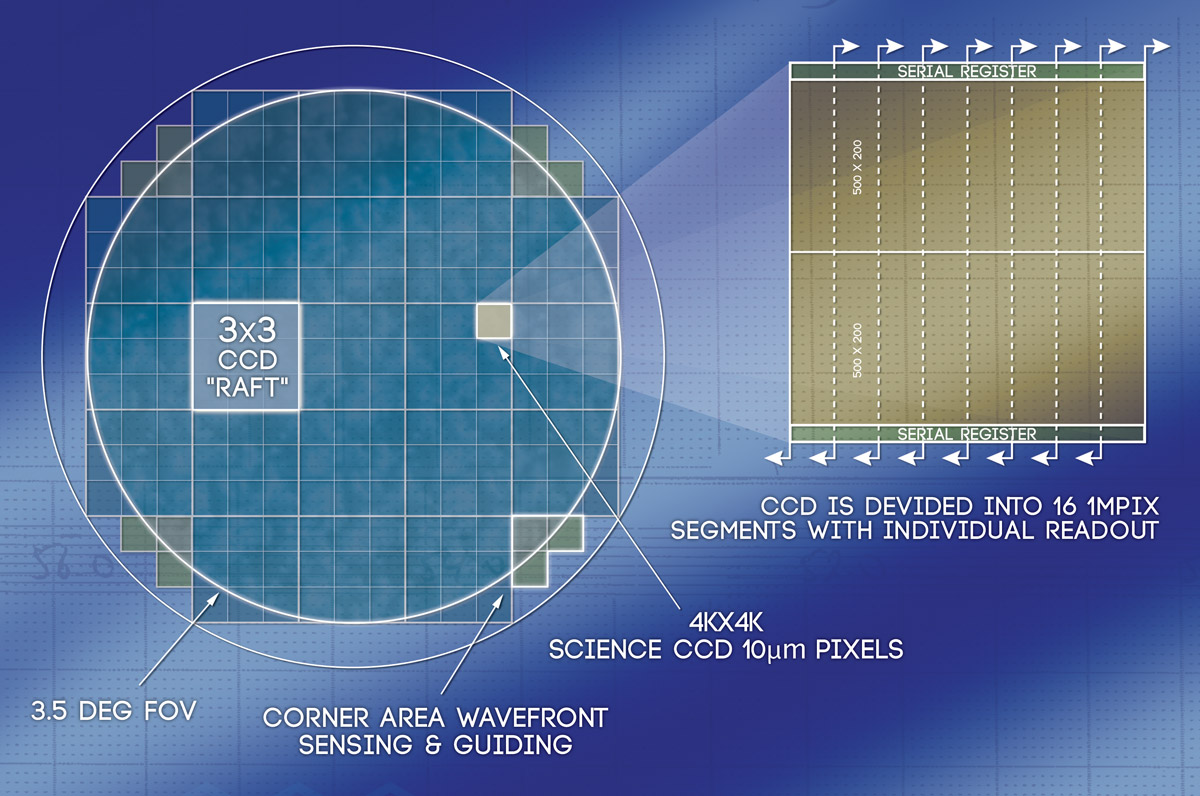
\includegraphics[width=0.9\textwidth]{LSST_FocalPlane_med.jpg}
            \newline
        \end{center}

    }

}


\frame
{
    \frametitle{Dark Energy Science Collaboration (DESC)}

    \setbeamerfont*{itemize/enumerate body}{size=\Large}
    \setbeamerfont*{itemize/enumerate subbody}{parent=itemize/enumerate body}
    \setbeamerfont*{itemize/enumerate subsubbody}{parent=itemize/enumerate body}
 
    \begin{itemize}

        \item Collaboration focused on Cosmology and Dark Energy from LSST

        \item Why is the expansion of the universe accelerating?

        \item Primary probes

            \begin{itemize}
                \item Weak Gravitational Lensing and Large Scale Structure
                \item Supernovae
                \item Clusters of galaxies
            \end{itemize}

        \item The main challenges involve image processing and simulations

    \end{itemize}

}

\frame
{
    \frametitle{Weak Gravitational Lensing}

    \setbeamerfont*{itemize/enumerate body}{size=\Large}
    \setbeamerfont*{itemize/enumerate subbody}{parent=itemize/enumerate body}
    \setbeamerfont*{itemize/enumerate subsubbody}{parent=itemize/enumerate body}
 
    \begin{itemize}

        \item Light is deflected as it passes massive objects, such as galaxies.

        \item The deflection distorts the images of galaxies behind the lens in a
            coherent way

        \item Can be used to measure the mass of objects in the universe, including Dark Matter

        \item Can be used to measure the effect of Dark Energy

    \end{itemize}

}

{

    \frame
    {
        \frametitle{Strong Lensing}
        \begin{center}
            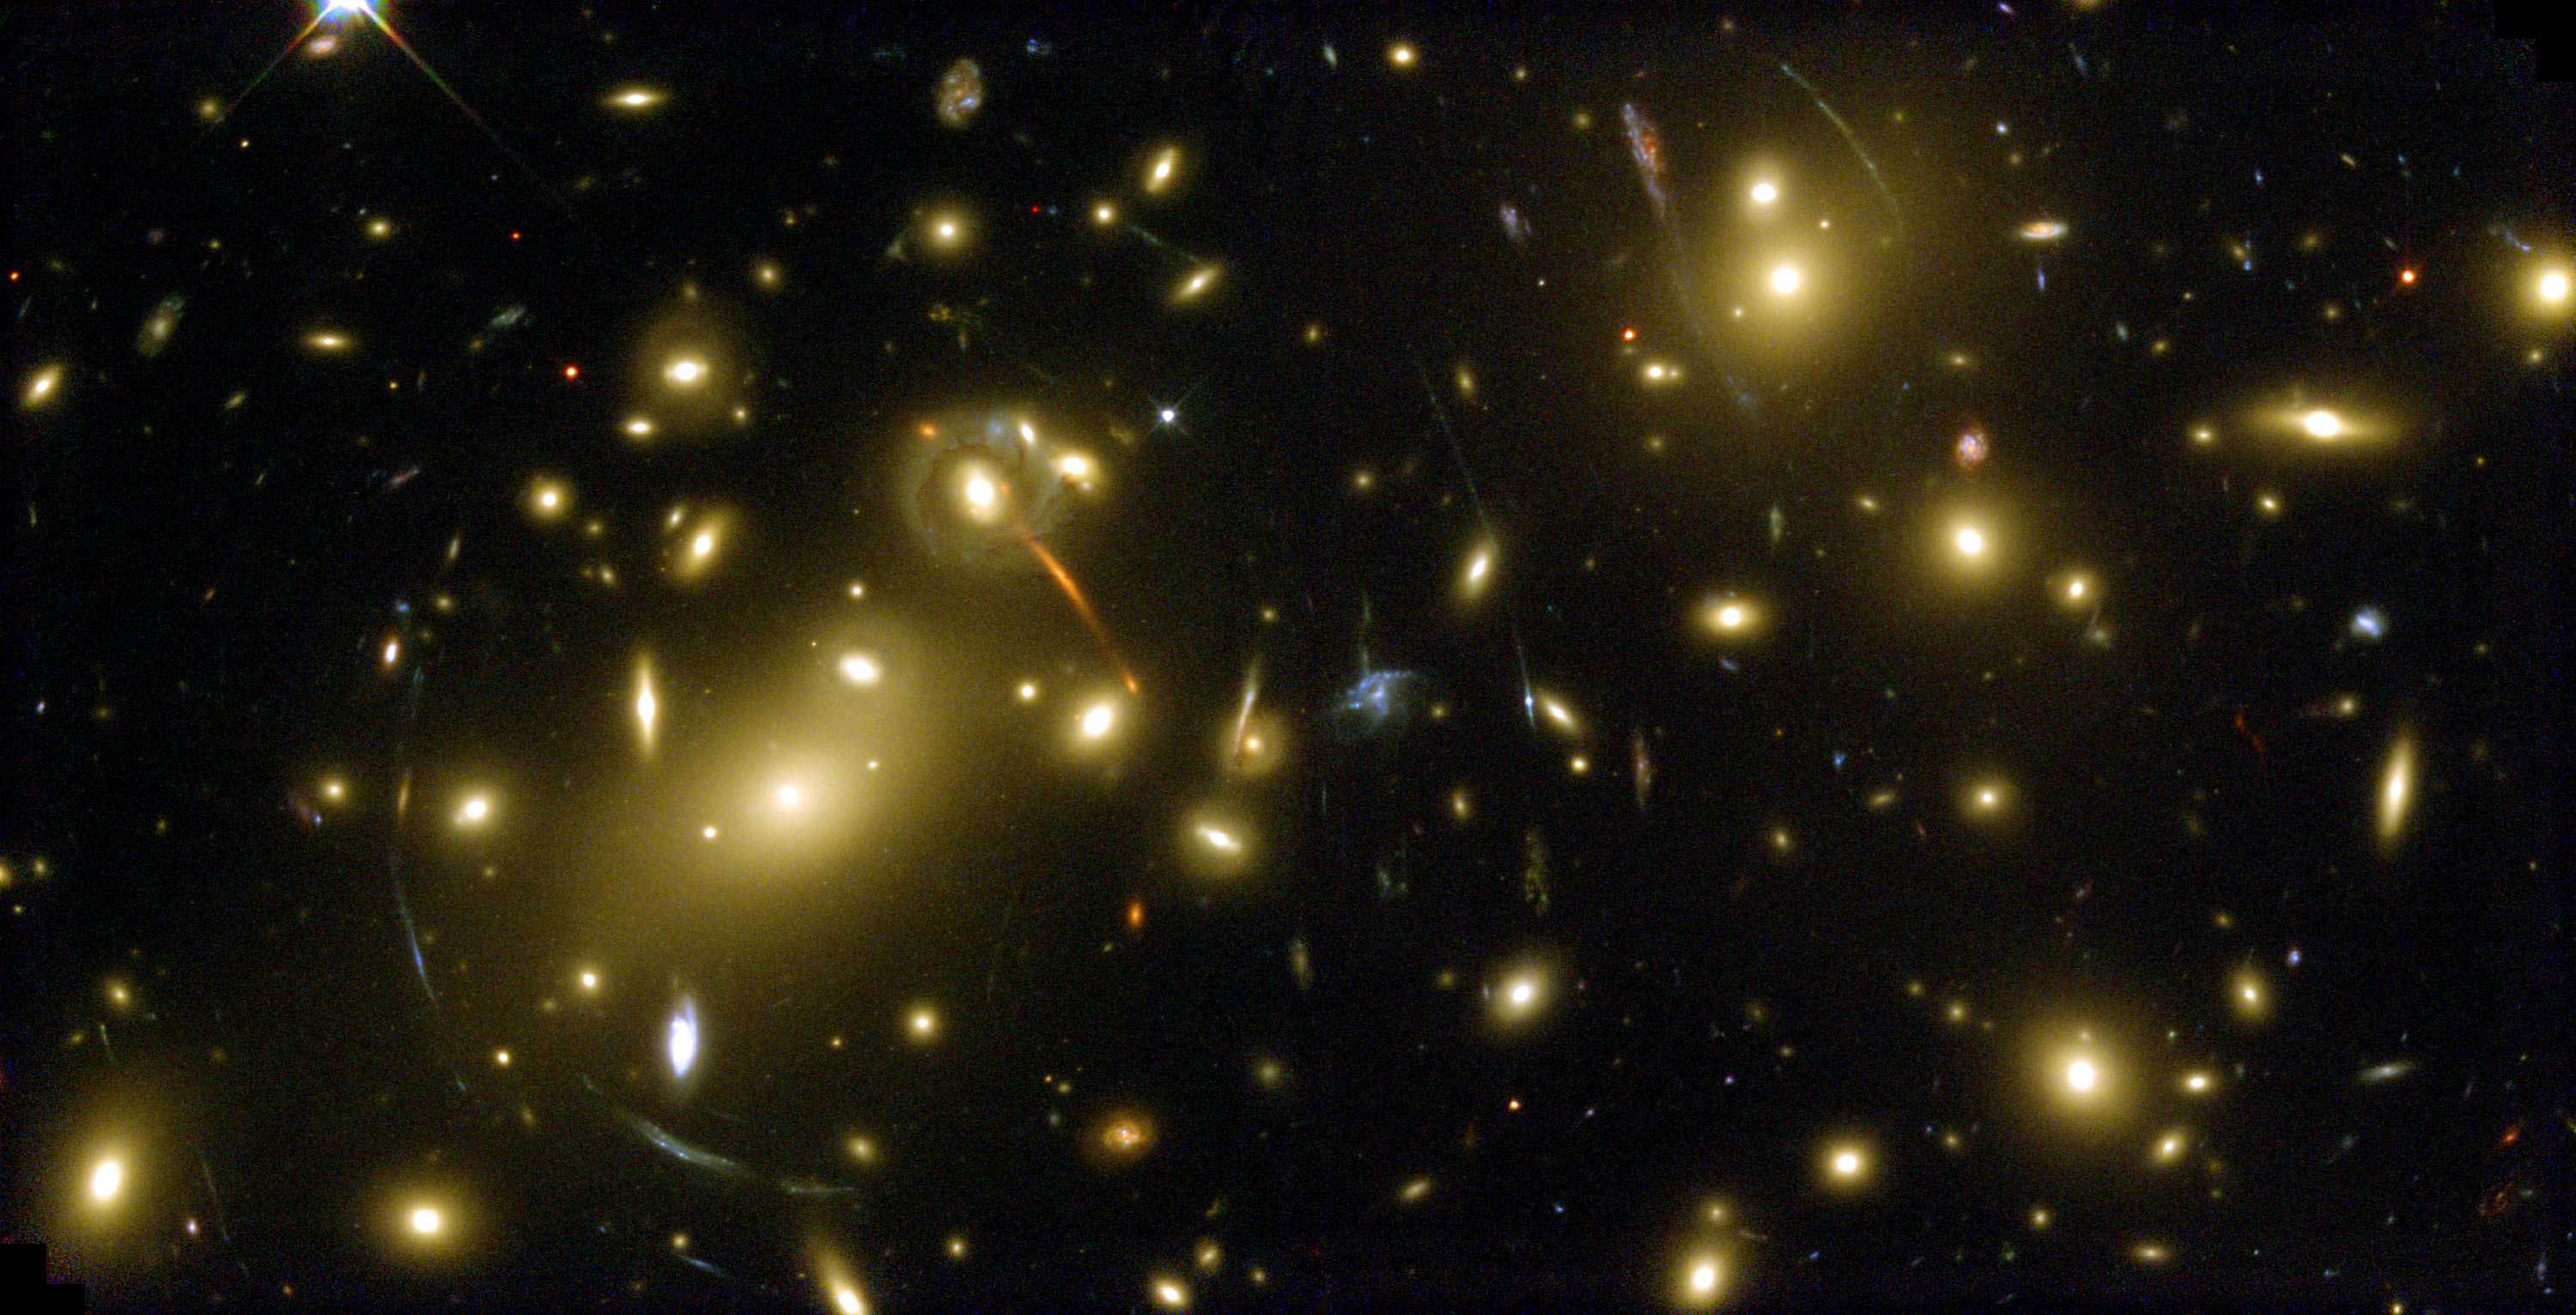
\includegraphics[width=1.0\textwidth]{abell2218.jpg}
            \newline
        \end{center}
        Weak lensing you can't see by eye, but it can be measured anywhere.

    }

}



\frame
{
    \frametitle{Computing Challenges for Weak Gravitational Lensing}

    \setbeamerfont*{itemize/enumerate body}{size=\large}
    \setbeamerfont*{itemize/enumerate subbody}{parent=itemize/enumerate body}
    \setbeamerfont*{itemize/enumerate subsubbody}{parent=itemize/enumerate body}
 
    \begin{itemize}


        \item The lensing effect changes the ellipticities of galaxies in a coherent way.
            Basic task is to measure ellipticities.

        \item There are many things that can bias the measurement: smearing by the atmosphere,
            optical distortions, noise, overlap of light from nearby objects.

        \item These are image processing challenges.
            
        \item We don't know how to do all these yet at the level required
            (0.1\%!).  This is still in {\color{gold} research!}

        \item Yet the success of LSST is depends on accurately measuring weak lensing.

    \end{itemize}

}

\frame
{
    \frametitle{Computational Challenges}

    \setbeamerfont*{itemize/enumerate body}{size=\large}
    \setbeamerfont*{itemize/enumerate subbody}{parent=itemize/enumerate body}
    \setbeamerfont*{itemize/enumerate subsubbody}{parent=itemize/enumerate body}
 
    \begin{itemize}

        \item Once algorithms are finalized, run on 60PB of images.

        \item But the algorithms are still in development.

        \item Testing the algorithms requires a huge amount of computing, because 
            most of the tests need to be done on the scale of the real survey.

        \item Testing also means running on the real data multiple times until
            systematic errors are reduced to required level

        \item Key Point:  We need a computing environment that supports
            development with quick feedback loops, as well as production runs,
            all with high throughput (basically the ATLAS/RHIC system at BNL
            is a perfect example).

    \end{itemize}

}

\frame
{
    \frametitle{Computational Challenges}

    %\setbeamerfont*{itemize/enumerate body}{size=\small}
    %\setbeamerfont*{itemize/enumerate subbody}{parent=itemize/enumerate body}
    %\setbeamerfont*{itemize/enumerate subsubbody}{parent=itemize/enumerate body}
 
    \begin{itemize}

        \item The DOE currently wants us to utilize NERSC

        \item NERSC is optimized for HPC: Massive production runs
            using proven codes.  Grab 100,000 cores in parallel.

        \item NERSC is a poor environment for our type of work and development.
            Even getting codes compiled requires expertise.  Getting running
            efficiently is a signifcant challenge even for experts
            
        \item You need to anticipate your work long in advance, submit job for
            huge number of cores, wait a week for the job to start, then once
            the job starts run your own queue on top of that job to spinoff
            each of the 1-core jobs.

        \item We need an automated system to make it easy to do development and
            production work without all this mental overhead.

        \item And remember we are a very diverse collaboration with many
            different code bases, science goals, and little HPC computing
            expertise.

    \end{itemize}

}



\frame
{
    \frametitle{Current Status with \panda}

    \setbeamerfont*{itemize/enumerate body}{size=\large}
    \setbeamerfont*{itemize/enumerate subbody}{parent=itemize/enumerate body}
    \setbeamerfont*{itemize/enumerate subsubbody}{parent=itemize/enumerate body}
 
    \begin{itemize}

        \item Heyun Park and I have begun working with Sergey and Pavlo at BNL.

        \item I have been able to run simple simulation jobs using \panda.

        \item Would like to get running on OSG since those are standard redhat
            systems.  Will take some learning curve to get started, but then
            developement work should be straightforward.

        \item Begin with simulations and processing data from pre-cursor survey
            DES (Dark Energy Survey).

        \item Eventually we may need work at NERSC through \panda.  Still need
            to compile codes on that system, and deal with non-standard
            environement, but hope \panda\ can simplify the work flow.

    \end{itemize}

}

\frame
{
    \frametitle{Time Scale}

    \setbeamerfont*{itemize/enumerate body}{size=\large}
    \setbeamerfont*{itemize/enumerate subbody}{parent=itemize/enumerate body}
    \setbeamerfont*{itemize/enumerate subsubbody}{parent=itemize/enumerate body}
 
    \begin{itemize}

        \item We will have ``first light'' engineering data in 2019, science
            data in 2021.

        \item We would like to have a standard system in place well before that, a system
            that makes it transparent to work on a variety of systems: OSG, NERSC, whatever
            is available.

        \item My goal would be to move all my processing to PanDA in a year.
            Would take longer to get others on board.

        \item Short term, process data from current surveys through the
            system.  Process LSST image simulations.

        \item Long term, process real LSST data.

    \end{itemize}

}






\end{document}
